%=========================Preamble====================================%
\documentclass[12pt] {article}
\usepackage{times}
\usepackage[margin=1in,bottom=1in,top=0.5in]{geometry}

\usepackage{graphicx}


\usepackage{float}
\usepackage{graphicx}
\usepackage{subfig}
\usepackage{wrapfig,lipsum}
\usepackage{amssymb}
\usepackage{nath}
\usepackage{amsfonts}


%=========================Doc====================================%
\begin{document}
\title{ECE 289A - An Introduction to Reinforcement Learning HW\#5}

\author{Ahmed H. Mahmoud}
\date{November, 16th 2017} 
\maketitle

\section*{Q.2}
Figure \ref{fig:b} shows the regenerate plot from Figure 9.10 in the book. 

\begin{figure}[!tbh]
\centering        
   \subfloat {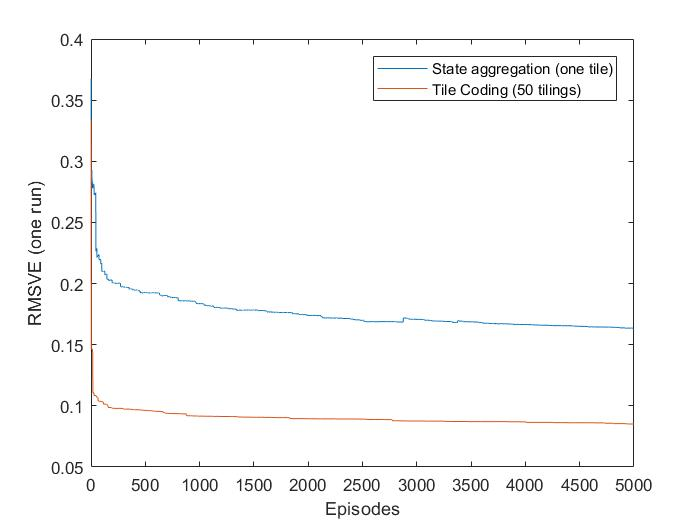
\includegraphics[width=0.9\textwidth]{fig9_10.jpg}}        
   \caption{Learning curve on the 1000-state random walk for gradient MC with a single tiling and multiple tilings.}
   \label{fig:b}
\end{figure}



\end{document}
